% THIS IS AN EXAMPLE DOCUMENT FOR VLDB 2012
% based on ACM SIGPROC-SP.TEX VERSION 2.7
% Modified by  Gerald Weber <gerald@cs.auckland.ac.nz>
% Removed the requirement to include *bbl file in here. (AhmetSacan, Sep2012)
% Fixed the equation on page 3 to prevent line overflow. (AhmetSacan, Sep2012)

\documentclass{vldb}
\usepackage{graphicx}
\usepackage{balance}  % for  \balance command ON LAST PAGE  (only there!)

\usepackage{setspace}
\usepackage{listings}
\lstset{frame=single, captionpos=b, escapeinside={<@}{@>}, numbers=left, mathescape=true}
\usepackage{xcolor}
\definecolor{bggray}{gray}{.95}

\hyphenation{Im-ple-men-tie-rungs-de-tails}
\hyphenation{Me-tho-de}

\begin{document}

% ****************** TITLE ****************************************

\title{Eine Architektur für grafische Benutzeroberflächen nach
dem MVC-Architekturmuster und unter Berücksichtigung
der SOLID-Architekturprinzipien}

\numberofauthors{1}
\author{
\alignauthor
Stefan Berger\\
       \affaddr{Beuth Hochschule für Technik Berlin}\\
       \affaddr{Luxemburger Str. 10}\\
       \affaddr{13353 Berlin}\\
       \email{s.berger@live.com}
}

\maketitle

\begin{abstract}
  Dieses Dokument befasst sich mit dem Model-View-Con\-trol\-ler (MVC) Architekturmuster. Es befasst sich weiterhin mit den fünf SOLID-Architekturprinzipien Single Responsibi\-lity, Open-Closed, Liskovsches Substitionsprinzip, Interface Segregation und Dependency Inversion. Das Architekturmuster wird auf die Architekturprinzipien hin überprüft und angepasst. In Beispiel\-implementierungen wird die Praxistauglichkeit nach den Anpassungen untersucht.

  Die Prinzipien werden einzeln für jede der drei Komonenten Model, View und Controller ausgewertet. Es sollen die Auswirkungen auf die Struktur einer MVC-Anwendung und die Anwendbarkeit bei der Entwicklung untersucht werden.

  Die neue Struktur bildet ein Grundgerüst, das aus den drei Komponenten des Architekturmusters sowie aus deren Unterkomponenten besteht. Die Komponenten und Unterkomponenten sind lose gekoppelt. Das Grundgerüst ist flexibel einsetzbar, stabil und erweiterbar.
\end{abstract}

\section{Introduction}
Seit der Entwicklung des Architekturmusters MVC hat sich in den Programmentwürfen für Benutzerschnittstellen die Trennung von Daten und Ansicht immer mehr durchgesetzt. Dabei wird der Quelltext einer Anwendung in die drei Klassen Programmlogik (Model), Ansicht (View) und Steuerung (Controller) unterteilt. Diese Struktur macht den Quelltext für Views und Controller austauschbar und wiederverwendbar. Außerdem erleichtern die Abstrahierung und die Modularisierung die Zusammenarbeit mehrerer Entwickler. Solange die Schnittstellen unverändert bleiben, können die verschiedenen Klassen flexibel und voneinander unabhängig bearbeitet werden.

Zwei der wichtigsten Argumente der SOLID-Prinzipien sind Wiederverwendbarkeit und Flexibilität. Außerdem soll durch deren Anwendung die Lesbarkeit und die Erweiterbarkeit des Quelltexts sichergestellt werden, und Entwicklerteams sollen effizienter zusammenarbeiten können. Die SOLID-Prinzipien sind in dem Buch ``Agile Software Development, Principles, Patterns, and Practices'' von Robert C. Martin ausführlich beschrieben.

Wir werden in den Abschnitten \ref{mvcsec} bis \ref{controllersec} zuerst die drei Komponenten des MVC-Architekturmusters und anschließend in den Abschnitten \ref{srpsec} bis \ref{dipsec} die fünf SOLID-Architekturprinzipien genau betrachten. Die drei Komponenten des MVC-Architekturmusters werden wir in den Abschnitten \ref{solidviewsec} bis \ref{solidmodelsec} jeweils auf die Relevanz der fünf SOLID-Prinzipien untersuchen und ent\-sprechend anpassen. In Bei\-spiel\-implementierungen werden wir die Praxis\-taug\-lich\-keit über\-prü\-fen.

\section{Architekturmuster und\\ Architekturprinzipien}
\subsection{MVC}
\label{mvcsec}
Das Architekturmuster MVC sieht für interaktive Anwendungen die Trennung in ein Modul für die Programmlogik (Model), ein Ansichtsmodul (View) und ein Steuerungsmodul (Controller) vor \cite[S.~26-49]{KraPo88}. Jedes dieser Module steht mit jedem anderen in einer bestimmten Relation.

\subsection{Model}
Im Model kann ein reines Datenmodell sein \cite[S.~27]{KraPo88} oder das Verhalten der Anwendung und das Datenmodell \cite[S.~2]{burbeck87}. Ein typisches Szenario ist eine Interaktion des Benutzers mit der View, die durch den Controller an das Model vermittelt wird. Bei jeder Änderung der Daten im Model benachrichtigt es die View. Die View aktualisiert schließlich die Darstellung der Daten. Danach oder auch währenddessen können weitere Interaktionen stattfinden.

Das Model ist normalerweise einzigartig, d.h. Views und Controller kennen nur ein Model. Model und View können jedoch mehrere verschiedene Datenobjekte austauschen \cite[S.~14]{Reens79}.

\subsection{View}
Eine Ansicht ist eine visuelle Repräsentation eines Models \cite[S.~1]{Reens79-1}. Die Relationen der drei Module werden durch verschiedene Entwurfsmuster realisiert. Die View als Observer des Mo\-dels \cite[S.~293—305]{GoF94} wird über Änderungen am Model benachrichtigt. Hierfür registriert die View einen oder mehrere Callbacks (Methoden oder Funktionen), die immer dann aufgerufen werden, wenn sich an den anzuzeigenden Daten etwas ändert. Man sagt, dass die View das Model kennt, das Model die View aber nicht – obwohl aus pro\-gram\-ma\-ti\-scher Sicht dem Model dadurch eine Schnittstelle der View bekannt gemacht wird. Mehrere Views können außerdem untereinander in Relation stehen. Mit dem Composite-Pat\-tern \cite[S.~163—175]{GoF94} können Teilkomponenten der View zum Gesamtmodul zusammengefasst werden. Sowohl das Gesamtmodul als auch die Teilkomponenten können dann auf Än\-de\-run\-gen am Model reagieren.

\subsection{Controller}
\label{controllersec}
Benutzereingaben werden vom Controller interpretiert. In Form des Strategy-Patterns \cite[S.~315—325]{GoF94} wird der View ein Controller zugewiesen. Eine View kann einen oder meh\-re\-re Controller besitzen. Normalerweise werden aber sogenannte View-Controller-Paare erzeugt, also eine View mit einem Controller. Der Controller der View kann sich je\-der\-zeit ändern, auch zur Laufzeit. Controller können außerdem die Fähigkeit besitzen, andere Views aufzurufen. Der Controller benötigt dann Zugriff auf ent\-spre\-chen\-de Schnittstellen der Laufzeitumgebung. Ein Controller muss außerdem das Datenmodell der Ansicht ma\-ni\-pu\-lie\-ren und diese aktualisieren können. %Wir sehen uns das in refinochwas genauer an.

\section{SOLID}
\subsection{Single Responsibility}
\label{srpsec}
Das Single-Responsibility-Prinzip besagt, dass es \textit{für eine Klasse nur einen Grund zur Änderung geben sollte} \cite[S.~63]{Martin17}. Nehmen wir an, dass eine Datenbankanwendung um eine Filtermöglichkeit nach betriebsspezifischen Kennzahlen -- etwa dem Anteil eines Verkaufsartikels am Umsatz -- erweitert werden soll. Um konkrete Werte für gefilterte Abfragen eingeben zu können, müssen der View entsprechende Steu\-er\-e\-le\-men\-te hinzugefügt werden. Jede Änderung, die außerdem an der View vorgenommen werden muss, weist auf eine Verletzung des Single-Responsibility-Prinzips hin.

Es ist zum Beispiel denkbar, dass der Ergebnistabelle im Viewmodul eine Spalte mit der neuen Kennzahl hinzugefügt werden soll. Offensichtlich müssen die Steuerelemente zur Eingabe der Abfragewerte und die Darstellung des Ab\-fra\-ge\-er\-geb\-nis\-ses in unterschiedlichen Viewklassen implementiert werden, sodass sichergestellt ist, dass jede Klasse eine einzige Verantwortlichkeit besitzt.

\subsection{Open-Closed}
Open-Closed sind \textit{Klassen, Module, Funktionen etc., die für Erweiterungen offen, aber für Modifikationen ver\-schlos\-sen sind} \cite[S.~99]{Marti13}. Ein Anwendungsgerüst muss flexibel erweiterbar sein, aber auch eine unveränderliche Grundfunktionalität bieten, die von Erweiterungen nicht beeinträchtigt wird.

Eine Hauptaufgabe von Controllerklassen ist es, Be\-nach\-rich\-ti\-gun\-gen entgegenzunehmen und weiterzuleiten. Weil die Stabilität des bestehenden Quelltexts davon abhängt, dass der Controller diese Aufgaben zuverlässig ausführt, muss die Controllerklasse für Änderungen an ihren Funktionen verschlossen sein.

Neue Controller-Implementierungen müs\-sen zusätzlich weitere Aufgaben ausführen. Das Modul muss deshalb für solche Erweiterungen offen sein.
\pagebreak

\subsection{Liskovsches Substitutionsprinzip}
Vereinfacht gesagt schreibt das Liskovsche Subs\-ti\-tu\-tions\-prin\-zip vor, dass \textit{Obertypen durch Untertypen ersetzbar sein} sollen \cite[S.~111]{Marti13}.

Angenommen, einer von mehreren Teil\-kom\-po\-nen\-ten des Viewmoduls soll ein Textfeld hinzugefügt werden. Die Teil\-kom\-po\-nente ohne das zusätzliche Textfeld soll aber weiterhin zur Verfügung stehen. Es ist naheliegend, für diesen Zweck eine neue Viewklasse von der bestehenden abzuleiten. Bei Bedarf kann dann ein Objekt der Basisklasse durch ein Objekt der abgeleiteten Klasse ersetzt werden.

Wird das Liskovsche Substitutionsprinzip befolgt, kann das Objekt der abgeleiteten Klasse verwendet werden, \textit{ohne das Viewmodul zu verändern}. Ein wichtiger Aspekt ist dabei das neue Datenfeld, das dem Viewmodul unbekannt sein muss.

\subsection{Interface Segregation}
Interface Segregation bedeutet, dass eine Klasse einer anderen genau die Schnittstelle zur Verfügung stellt, die für den jeweiligen Zweck vorgesehen ist.

Im MVC-Architekturmuster verwenden sowohl die View als auch der Controller Schnittstellen des Models. Die View muss als Empfänger für Benachrichtigungen über Än\-de\-run\-gen registriert werden. Der Controller muss das Model über Benutzereingaben benachrichtigen. Daraus ergeben sich zwei verschiedene Schnittstellen zum Model. Gemäß des Interface-Segretation-Prinzips sollten die View und der Controller auch zwei verschiedene Schnittstelle erhalten.

\subsection{Dependency Inversion}
\label{dipsec}
Das Dependency-Inversion-Prinzip schreibt vor, dass Mo\-dule nicht von anderen Modulen, die sich niedriger in der Modulhierarchie befinden, abhängig sein sollten \cite[S.~127]{Marti13}.

Wir werden dieses Prinzip bei der Implementierung des Viewmoduls und seiner Teilkomponenten berücksichtigen.

\section{SOLID View}
\label{solidviewsec}
\subsection{Single Responsibility im Viewmodul}
Ein Viewmodul beinhaltet wenig bis keine Programmlogik. Es re\-a\-giert auf Änderungen an den Anwendungsdaten und macht diese sichtbar.

Für Benachrichtigungen über Änderungen ist das Obser\-ver-Entwurfsmuster vorgesehen. Ein Observer hat eine Verantwortlichkeit im Sinne des Single-Re\-spon\-si\-bi\-li\-ty-Prinzips. Die Registrierung am Model und der Callback sollten sich deshalb in einer eigenen Klasse befinden.

\begin{figure}[h]
  \centering
  \includegraphics[scale=.95]{view-1.mps}
  \caption{Klassendiagramm des Viewmoduls}
  \label{viewmps}
\end{figure}

Abbildung \ref{viewmps} zeigt die Klassenstruktur des Viewmoduls. Die Klasse \texttt{DateTimeObserver} erhält Benachrichtungen über Änderungen im Datenmodell der Anwendung und leitet sie an Objekte der Klasse \texttt{DateTimeView} weiter.

Die Klasse \texttt{View} ist für die Darstellung der Daten und Zustände verantwortlich. Diese Klassenstruktur befolgt das Single-Responsibility-Prinzip besser als eine einzige \texttt{View}-Klasse, in der alle diese Aspekte implementiert sind.

\subsection{Open-Closed im Viewmodul}
Die Klasse \texttt{DateTimeObserver} ist für Modifikationen am zugrundeliegenden Observer-Entwurfsmuster verschlossen. Um zum Beispiel mehrere Ansichten über Änderungen am Modul zu informieren ist sie Erweiterungen am Be\-nach\-rich\-ti\-gungs\-me\-cha\-nis\-mus sie da\-ge\-gen offen.

Die Klasse \texttt{DateTimeView} ist für Erweiterungen an ihrer Prä\-sen\-ta\-tions\-lo\-gik offen. Die Methoden \texttt{show} und \texttt{update} können zu diesem Zweck überschrieben werden. Die Implementierung des Composite-Entwurfsmusters der abstrakten Basisklasse \texttt{CompositeView} ist für Modifikationen verschlossen.

Es sind keine Än\-de\-run\-gen am Ansichtsmodul nötig, um neue Ansichten zu implementieren. Die Vorgaben des Open-Closed-Prinzips sind eingehalten.

\subsection{Liskovsches Substitionsprinzip im Viewmodul}
Das Viewmodul des Grundgerüstes besitzt keine Ver\-er\-bungs\-hie\-rar\-chie. Für die Erweiterungen des Datenmodells und der Prä\-sen\-ta\-tions\-lo\-gik werden von den bestehenden Klas\-sen neue ab\-ge\-lei\-tet.

Nennen wir eine Klasse zur Verwaltung unserer Ansichten, welche die Interfaces \texttt{View} und \texttt{Updatable} implementiert, \texttt{CompositeView}. Eine Ansicht besteht aus verschiedenen Ele\-men\-ten, die alle bei Aktualisierungen der Daten benach\-richtigt werden müssen. Das Programm über\-gibt Informationen darüber, welche Daten dargestellt werden sollen, an die Methode \texttt{update} des Interfaces \texttt{Updatable} im Para\-meter \texttt{appState}. \texttt{CompositeView} erhält zwei weitere Methoden \texttt{addChild} und \texttt{getChildren}, mit denen Unteransichten organisiert werden können.

Wir fügen der Klasse \texttt{CompositeView} eine Erweiterung hinzu, indem wir eine neue Klasse ableiten. Wir nennen die Klasse \texttt{DateTimeView}. Mit ihr werden das Datum und die Uhrzeit dargestellt, indem jeweils eine Unteransicht hinzu\-gefügt wird. Für die Unteransichten werden die Klassen \texttt{DateView} und \texttt{TimeView} von \texttt{CompositeView} abgeleitet. Die Methode \texttt{update} in \texttt{DateTimeView} be\-kommt im Parameter \texttt{appState} die Bestandteile des Datums und der Uhrzeit als Ganzzahlen übergeben. Die Methode wird über\-schrieben, um die Basisklassenversion aufzurufen, in der die Unteransichten ebenfalls aktualisiert werden. In \texttt{appState} sind in einer generischen Map die Daten der verschiedenen Ansichten, also Datum und Uhrzeit, separat abgelegt. Dadurch behält der Parameter aller \texttt{update}-Methoden der verschiedenen Ansichts\-klassen denselben Typ.

Objekte der Klasse \texttt{DateTimeObserver} funktionieren zu\-sammen mit Objekten der Klasse \texttt{DateTimeView}, die direkt von der abstrakten Basisklasse abgeleitet ist, genauso wie mit Objekten der Klassen \texttt{DateView} und \texttt{TimeView}, die von der konkreten Implementierung erneut abgeleitet wurden. Die Forderung des Liskovschen Substitutionsprinzips ist erfüllt.

\subsection{Interface Segregation im Viewmodul}
Das Interface \texttt{View} stellt die Methode \texttt{show} zur Verfügung, um die Ansicht initial darzustellen. Ein Objekt der Klasse \texttt{DateTimeObserver} erhält eine Referenz auf die Hauptansicht in Form eines Attributes vom Typ \texttt{Updatable}. Die Klasse \texttt{CompositeView} implementiert die einzige Methode \texttt{update} dieses Interfaces und die Methode \texttt{show}. Der Implementierung des Interfaces \texttt{Clock}, welche die eigentliche Arbeit verrichtet, ist zu diesem Zweck ebenfalls nur die Methode \texttt{update} des Interfaces \texttt{Observer} bekannt. Die klar definierten Schnittstellen für jede Beziehung zwischen den Komponenenten erfüllt die For\-de\-rung des In\-ter\-face-Seg\-re\-ga\-tion-Prinzips.

\subsection{Dependency Inversion im Viewmodul}
Die Klassen, die direkt oder indirekt das Interface \texttt{View} implementieren, stellen die ``High Level Modules'' des Viewmoduls im Sinne des Dependency-Inversion-Prinzips dar. Das Prinzip besagt, dass diese Klassen nicht von Implementierungsdetails in den anderen Klassen abhängig sein dürfen. Dadurch soll verhindert werden, dass Änderungen an Im\-ple\-men\-tie\-rungs\-de\-tails die Geschäftslogik insgesamt beein\-trächtigen. Wie schon beim Open-Closed-Prinzip ermöglicht Abstraktion, diese Anforderung zu erfüllen. Alle Attribute der Klasse \texttt{CompositeView} und der von \texttt{CompositeView} ab\-gelei\-teten Klassen sind vom Typ eines Interfaces. Die Implementierungsdetails befinden sich in abgeleiteten Klassen, oh\-ne die un\-ge\-wünsch\-te Abhängigkeit zu erzeugen.

\section{SOLID Controller}
\subsection{Single Responsibility}
Der Controller in einer MVC-Anwendung hat zwei Aufgaben. Er interpretiert Benutzereingaben und er be\-nach\-rich\-tigt andere Module über relevante Be\-nut\-zer\-ein\-ga\-ben. Hier\-für hält er gegebenenfalls Zustandsdaten der Ansicht vor.

\begin{figure}[h]
  \centering
  \includegraphics[scale=.95]{controller-1.mps}
  \caption{Klassendiagramm des Controllermoduls}
  \label{controllermps}
\end{figure}

Im Beispiel der Ansichtsklasse \texttt{DateTimeView} besitzen die beiden Unteransichten \texttt{DateView} und \texttt{TimeView} jeweils einen Controller. Jeder der beiden Controller besitzt ein Attribut, in dem Benutzereinstellungen zum Format der Datums- oder Zeitanzeige vorgehalten werden und ein Attribut vom Typ \texttt{UpdateService}, mit dem die Neuberechnung der an\-zu\-zei\-gen\-den Daten im Fall einer entsprechenden Änderung der Einstellungen durch den Benutzer angestoßen werden kann.

Da\-für ist eine Methode \texttt{getMouseEventHandler} im Interface \texttt{Con\-troller} festgelegt, die einen Event-Handler für die je\-wei\-li\-ge Ansichtsklasse erzeugt und zurückgibt. Die Klassen \texttt{DateController} und \texttt{TimeController} implementieren diese Methode ihren Anforderungen entsprechend.

Durch die Aufteilung der zwei Aufgaben auf die zwei verschiedenen Interfaces \texttt{Controller} und \texttt{UpdateService} kann es für Änderungen an deren Implementierungen immer nur einen einzigen Grund geben. Das Single-Responsibility-Prin-zip also eingehalten.

\subsection{Open-Closed im Controllermodul}
Im Controllermodul befindet sich zwei Implementierungen des Interfaces \texttt{Controller}. Sie erstellen Event-Handler für die Ansichtsklassen. Sie besitzen jeweils ein Attribut vom Typ \texttt{UpdateService} und sind für Änderungen an diesem Attribut verschlossen.

Die Methode \texttt{getMouseEventHandler}, in der das Verhalten bei Klicks des Benutzers definiert wird, ist für Änderungen offen.

Die Klasse \texttt{DateTimeUpdateService} besitzt zwei un\-ver\-än\-der\-li\-che Attribute, und zwar die Schnittstellen zur Ansicht und zur Hauptanwendung. Diese Methode ist als nicht überschreibbar deklariert, um die Forderungen des Open-Closed-Prinzips zu erfüllen.

\subsection{Liskovsches Substitutionsprinzip\\im Controllermodul}
Es gibt im Controllermodul wie auch im Viewmodul zu\-nächst keine Vererbungshierarchie. Erweitern wir die Implementierungen der Interfaces, sind die Forderungen des Liskovschen Substitutionsprinzips einzuhalten.

Um dem Anwender die Möglichkeit zu bieten, Datum und Uhrzeit per Drag-and-Drop im Anwendungsfenster zu verschieben, kann eine Implementierung des Interfaces \texttt{Con\-troller} erstellt werden, die statt einem \texttt{MouseListener} ei\-nen \texttt{MouseInputListener} zurückgibt. Eine Spe\-zia\-li\-sie\-rung des Typs der Interface-Methode ist mit dem Liskovschen Substitutionsprinzip vereinbar, eine Basisklasse dürfte hier nicht verwendet werden. In der Parameterliste ist es um\-ge\-kehrt, dort dürften die Typen nur in allgemeinere geändert werden.

In der Schnittstelle der Klasse \texttt{Controller} sind keine Über\-gabeparameter deklariert. Das Liskovsche Substitutions\-prinzip ist eingehalten, wenn die Schnittstelle wie be\-schrie\-ben oder gar nicht verändert wird.

\subsection{Interface Segregation im Controllermodul}
Das Controllermodul ist außer der Hauptanwendung nur dem Ansichtsmodul bekannt. Die Ansicht nutzt die Methode \texttt{getMouseEventHandler} des Interfaces \texttt{Con\-troller}, um auf Benutzereingaben zu re\-agie\-ren.

Die beiden Implementierungen des Interfaces \texttt{Controller} besitzen als Attribut einen \texttt{UpdateService}, der für Nach\-rich\-ten an die Hauptanwendung über Änderungen durch den Benutzer verantwortlich ist.

Die Klasse \texttt{UpdateService} erhält eine Schnittstelle der Hauptansicht vom Typ \texttt{Clock}, denn sie benötigt nur eine Me\-thode, um die Anwendung zu veranlassen, den \texttt{appState} neu zu berechnen. Durch diese Trennung der Ver\-ant\-wort\-lich\-kei\-ten sind die Anforderungen des Interface-Segregation-Prinzips auch im Controllermodul erfüllt.

\subsection{Dependency Inversion im Controllermodul}
Wie in Abschnitt \ref{dipsec} angedeutet, ist Dependency Inversion in MVC-Architekturen vor allem im Viewmodul zu be\-ach\-ten. Das Controllermodul definiert zwar auch eine Ab\-hän\-gig\-keit der Klasse \texttt{Controller} von \texttt{UpdateService}. Weil \texttt{UpdateService} eine abstrakte Klasse ist, wird die Dependency Inversion dadurch aber bereits sichergestellt.

\section{SOLID Model}
\label{solidmodelsec}
\subsection{Single Responsibility}
Das Model im MVC-Architekturmuster ist noch etwas abstrakter als die anderen Komponenten. View und Controller dienen in MVC immer demselben Zweck, während die Funktion des Models von der Art der Anwendung abhängt. Zum Beispiel verwaltet eine Notizbuch-Anwendung eine Sammlung von Notizen, und hält eine unbestimmte Anzahl Notizen im Arbeitsspeicher vor. Eine Anwendung für Online-Banking berücksichtigt dagegen vor allem Sicherheitsaspekte und kann erfolglose Transaktionen rückabwickeln.

\begin{figure}[h]
  \centering
  \includegraphics[scale=.95]{model-1.mps}
  \caption{Klassendiagramm des Models}
  \label{modelmps}
\end{figure}

Das Model ist ein generischer Container für die Daten, die in der Ansicht dargestellt werden sollen. Dadurch ist es unter anderem möglich, der Ansicht die verschiedenartigen Datenstrukturen der verschiedenen Unteransichten in einem einzigen Aufruf zu übermitteln.

Das Model im MVC-Architekturmuster besitzt bereits die einzige Verantwortlichkeit, der Ansicht aktuelle Daten bereitzustellen. Wird diese Verantwortlichkeit mittels Observer-Entwurfsmuster realisiert, ist das Single-Responsibility-Prin\-zip eingehalten.

\subsection{Open-Closed im Model}
Die Nachrichtenübermittlung vom Controller an das Model und vom Model an die View sind essentielle Bestandteile des Models. Sie sind verschlossen für Veränderungen. Die sekündliche Aktualisierung der Daten ist ebenfalls für Modifikationen verschlossen. Dasselbbe gilt für die Benachrichtigungen des Observers im Ansichtsmodul.

Die Berechnung der Daten ist für Erweiterungen offen. Denkbare Erweiterungen sind die Berechnung der Weltzeit und länderspezifische Datums- und Zeitformate. Das Open-Closed-Prinzip ist in der DateTime-Anwendung eingehalten.

\subsection{Liskovsches Substitutionsprinzip im Model}
Das Model der DateTime-Anwendung ist in einer flachen Klassenhierarchie gehalten. Das Substitutionsprinzip wird deshalb für das Model auch nicht verletzt.

Theoretisch denkbar wäre eine Klasse, die beispielsweise statt nur einer Uhrzeit die Weltzeit an die Ansicht über\-mit\-telt. Eine Spezialisierung dieser Klasse könnte die Zugriffsmethoden überschreiben, die in der Basisklasse für ein Objekt einer Zeitzonenkonfigurationsklasse, bestehend aus Land und Stadt, die Uhrzeit in einem Objekt einer ebenfalls hierfür erstellten Klasse zurückgibt. In der Überschreibung könnten zusätzlich die jährlichen Zeitumstellungen be\-rück\-sich\-tigt werden.  Um das Liskovsche Substitutionsprinzip einyuhalten dürfte hierfür der Parameter der Zu\-griffs\-me\-tho\-de nicht in einen spezielleren Typ geändert werden. Der Rückgabetyp dürfte nicht in einen allgemeineren Typ ge\-än\-dert werden.

\subsection{Interface Segregation im Model}
Das Model ist dem Controllermodul in Form des Interfaces \texttt{Clock} bekannt. Das Interface bietet dem Controller durch die Methode \texttt{tick} die Möglichkeit, die berechneten Daten zu aktualisieren.

Das Model kennt nur den Observer des Ansichtsmoduls. Das Interface \texttt{Observer} stellt die Methode \texttt{notify} bereit, mit welcher die Ansicht über geänderte Daten benachrichtigt wird.

Die Ansicht kennt das Datenmodell. Es besteht aus reinen Datenobjekten für Datum und Uhrzeit und einer Map zur Organisation der Daten nach Unteransicht. Mit dieser Trennung der Schnittstellen nach den jeweiligen Anforderungen der Komponenten wird das Interface-Segregation-Prinzip be\-rück\-sich\-tigt.

\subsection{Dependency Inversion im Model}
Das Model ist das Modul der DateTime-MVC-Anwendung mit den meisten Abhängikeiten. Es erstellt die Ansichten und die zugehörigen Controller, erlaubt dem Controller das Aktualisieren der Daten und stellt der View das Datenmodell in einem generischen Container bereit.

Für alle diese Abhängigkeiten zum und vom Model wurden Interfaces genutzt. Das Dependency-Inversion-Prinzip ist dadurch eingehalten.

\section{Experiment}
Um das Grundgerüst auf seine Praxistauglichkeit zu testen wurde die DateTime-Anwendung entwickelt. Sie zerlegt die Systemzeit in ganzzahlige Bestandteile, um sie als Datenmodell den Ansichten zur Verfügung zu stellen.

Im untenstehenden Listing ist zu erkennen, dass eine Datenmodellklasse für den Datumsteil und eine für den Uhrzeitteil existiert. Die beiden Klassen entsprechen den beiden Unteransichten im Ansichtsmodul.

Die Unteransichten besitzen jeweils einen Controller. Bei Klick auf eine der Ansichten werden die Formatoptionen geändert, deren Klassen ebenfalls im untenstehenden Listing verwendet werden. Die Objekte für die Formatoptionen werden im Controller referenziert. Dort werden die Eigenschaften in den Ereignisbehandlungsroutinen geändert und im Model wird die Neubberechnung des Datums und der Uhrzeit veranlasst. Schließlich wird der Observer im Ansichtsmodul über die Änderungen informiert.

\begin{small}
\setstretch{1.0}
\begin{lstlisting}[language=Java, caption=Das Model der Anwendung, label=list:contractcontroller]
public void tick() {
  Calendar calendar =
    GregorianCalendar.getInstance();

  dateAppState.year =
    calendar.get(Calendar.YEAR);
  dateAppState.month =
    calendar.get(Calendar.MONTH);
  dateAppState.day =
    calendar.get(Calendar.DATE);
  if (dateFormatOptions.longMonth) {
    dateAppState.month = -1;
    dateAppState.monthName =
      Month.of(calendar.get(Calendar.MONTH))
        .toString();
  } else {
    dateAppState.month =
      calendar.get(Calendar.MONTH);
    dateAppState.monthName = "";
  }

  timeAppState.seconds =
    calendar.get(Calendar.SECOND);
  timeAppState.minutes =
    calendar.get(Calendar.MINUTE);
  if (timeFormatOptions.twentyFourHours) {
    timeAppState.amPm = "";

    if (calendar.get(Calendar.AM_PM) ==
      Calendar.PM) {
        timeAppState.hours =
        calendar.get(Calendar.HOUR) + 12;
    }
  } else {
    timeAppState.hours =
      calendar.get(Calendar.HOUR);
    timeAppState.amPm =
      calendar.get(Calendar.AM_PM) ==
        Calendar.AM ? "am" : "pm";
  }

  appStateContainer.registerClass(
    DateAppState.class, dateAppState);
  appStateContainer.registerClass(
    TimeAppState.class, timeAppState);

  observer.notify(appStateContainer);
}

\end{lstlisting}
\end{small}

\section{Fazit}
Das Einhalten der SOLID-Prinzipien beim Entwurf einer MVC-Architektur führt zu komplexen Klassendiagrammen der einzelnen Komponenten. Dafür entkoppelt es die Komponenten und auch die Unterkomponenten und ermöglicht eine einfache Erweiterung der verschiedenen Module.

\begin{figure}[h]
  \centering
  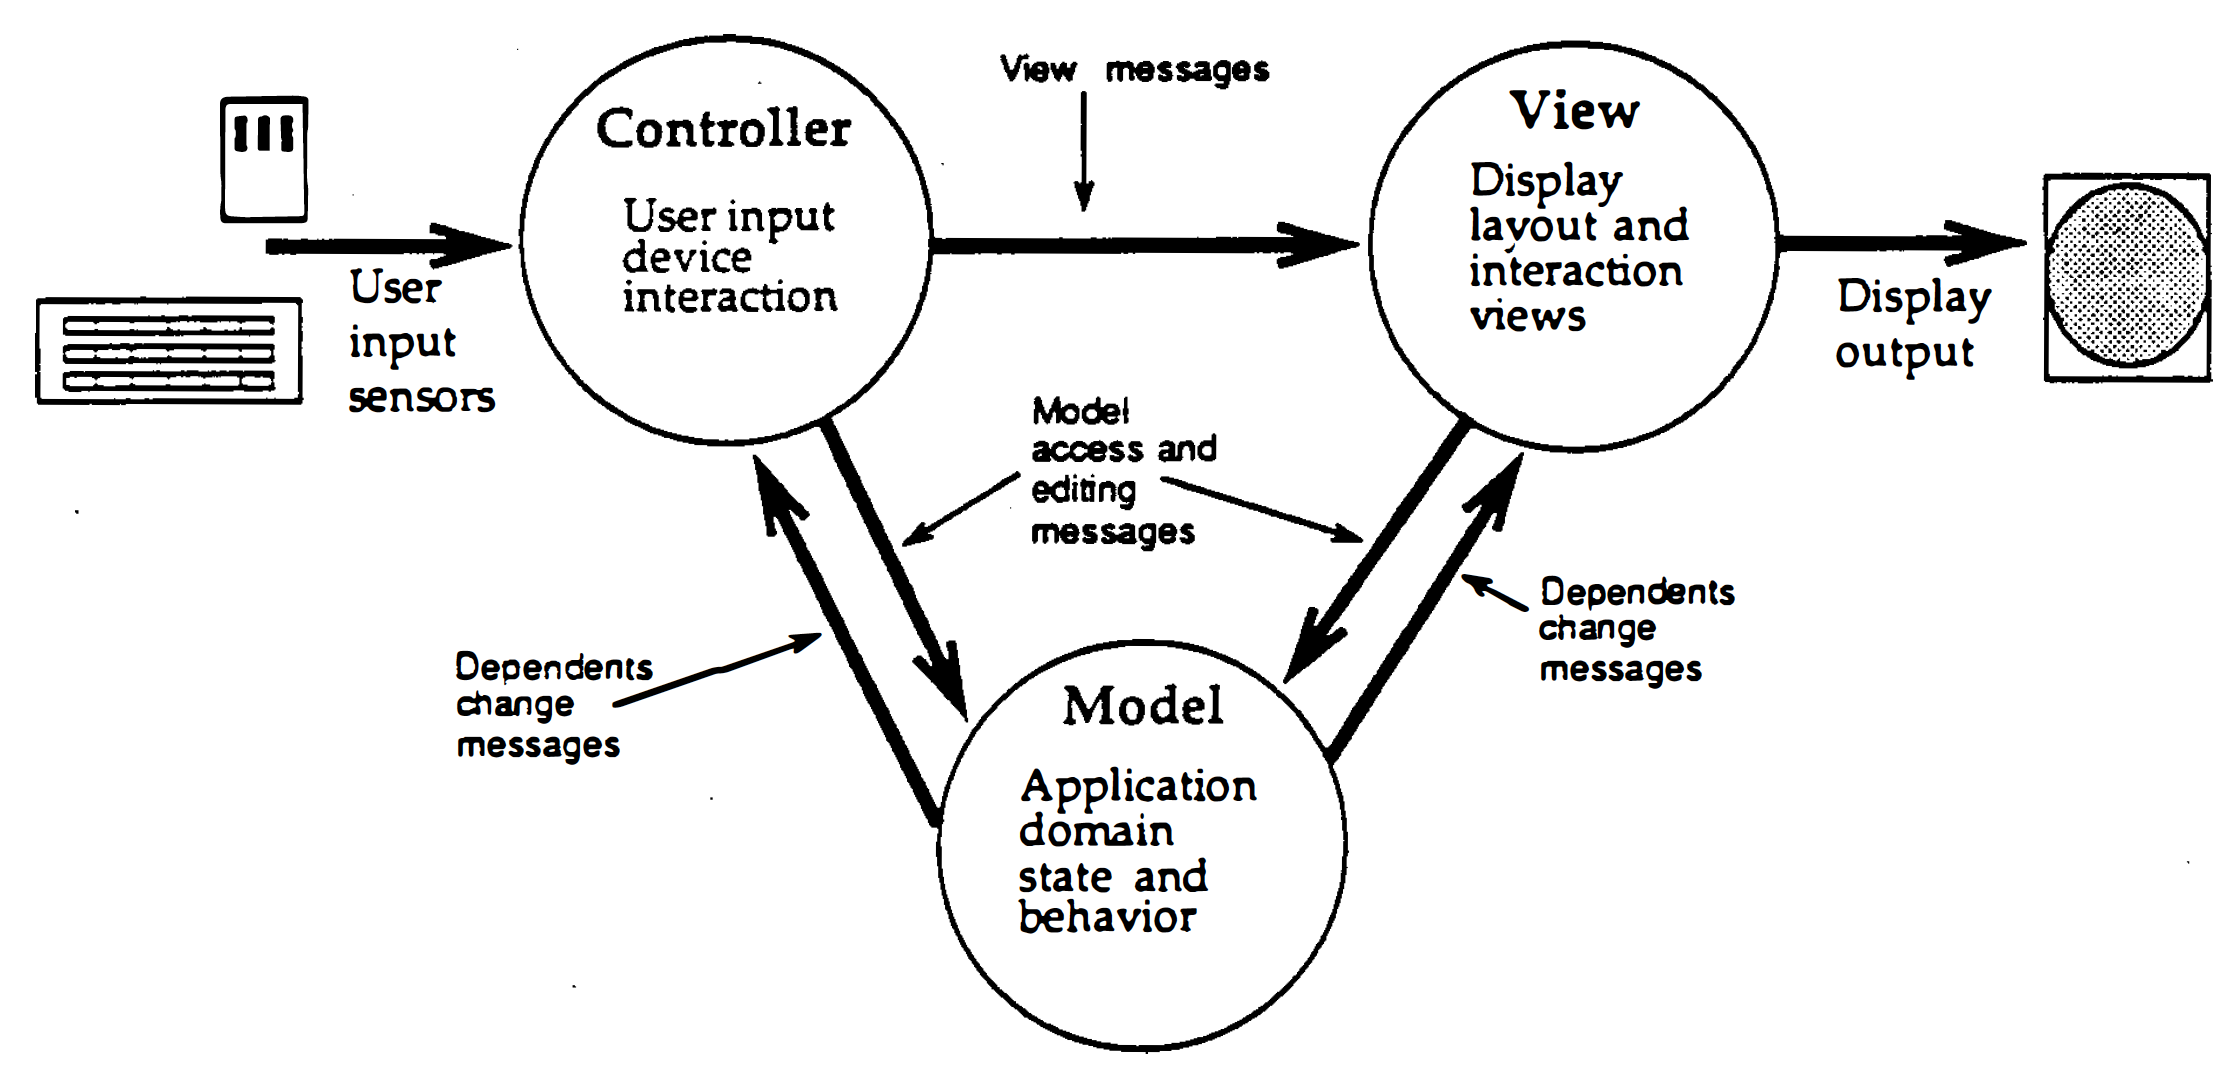
\includegraphics[scale=.15,natwidth=1350,natheight=700]{diagram.png}
  \caption[caption]{Typisches MVC-Diagramm \cite[S.~27]{KraPo88}}
  \label{diagram}
\end{figure}

Durch Abstraktionen wird der Controller beispielsweise vom Service zum Aktualsieren der Modeldaten entkoppelt. Die Aus\-tausch\-bar\-keit der Kompenenten wird dadurch erhöht, und die Ab\-hän\-gig\-keiten werden auf ein Minimum reduziert \cite[S.~2]{Liskov1987}.

Das Model wurde durch die neue Architektur besonders stark umgestaltet. Im Einsprungspunkt in der Hauptklasse werden zunächst alle MVC-Module initialisiert. Die Controller werden an die Ansichten und die Ansichten an das Model gekoppelt, und das Datenmodell wird auf die Über\-tragung an die Ansicht vorbereitet.

In der Ansicht ist nun der Observer für die Modeldaten von dem Konstrukt des Composite-Patterns für die Haupt- und Unteransichten völlig losgelöst. Die Ansichtsklassen implementieren zwei verschiedene Interfaces, um dem Observer und dem Composite-Pattern jeweils die Richtige Schnittstelle anzubieten.

Das Single-Responsibility-Prinzip hat den größten Einfluss auf die MVC-Architektur. Diagramme des MVC-Ar\-chi\-tek\-tur\-mus\-ters %\#refs\#refs\#refs
zeigen normalerweise die drei Komponenten Model, View und Controller und nennen keine weiteren Klassen (siehe Abbildung \ref{diagram}).

Durch die Beschränkung einer Klasse auf genau eine Verantwortlichkeit erweitert sich das Model auf mindestens zwei Klassen für Nachrichten des Controllers und das Datenmodell. Aufgrund der anderen SOLID-Prinzipien sind es sogar drei Interfaces.

Die Ansicht besteht wegen des Single-Responsibility-Prin\-zips mindestens aus einer Observerklasse für Modeldaten und einer Klasse für das Composite-Pattern. Wie auch beim Model sind es in Wirklichkeit drei Interfaces.

Das Controllermodul besteht nun aus zwei Unterkomponenten, nämlich aus dem Controller für die Ereignisbehandlung der Ansicht und dem UpdateService für die Kommunikation mit dem Model.

Die Gesamtarchitektur besteht nun aus sechs statt vorher drei (Unter-)Komponenten.

Das Open-Closed-Prinzip zwingt uns, die neue Architektur als Gesamtheit zu betrachten. Für das architektonische Grundgerüst war zu beachten, dass bestimmte Eigenschaften einer MVC-Anwendung immer vorhanden sein müs\-sen, andere Eigenschaften aber nur für bestimmte Anfor\-de\-run\-gen zu implementieren sind. Die Architektur kann um diese anderen Eigenschaften erweitert werden, ohne die Komponenten zu verändern.

Die DateTime-Anwendung erstellt keine Views ohne Controller und tauscht den Controller einer View auch nie aus. Diese Eigenschaften können jedoch implementiert werden, ohne das Grundgerüst zu verändern.

Das Composite-Pattern ist fest in der Ansicht verankert. Das Datenmodell ist flexibel genug, um jeder Unteransicht eine eigene Klasse für Daten zu ermöglichen, und diese Eigenschaft ist ebenfalls verschlossen für Modifikationen.

Wir haben das  Liskovsche Substitutionsprinzip beim Entwurf des Datenmodells berücksichtigt. Es ist ein generischer Container für alle denkbaren Datenmodelle und muss deshalb nicht spezialisiert zu werden. Dadurch kann das Model in jeder abgeleiteten Viewklasse unverändert als Über\-gabe\-para\-meter verwendet werden.

Das Grundgerüst besitzt ansonsten nur eine flache Hie\-rar\-chie, die aus Interfaces und wenigen Klassen besteht. Diese kann das Liskovsche Substitutionsprinzip nicht verletzen. Das Prinzip kann aber in Anwendungen berücksichtigt werden, die das Grundgerüst nutzen und die Interfaces implementieren.

Interface Segregation ist das zweite Prinzip, das er\-heb\-li\-chen Einfluss auf die Struktur der neuen MVC-Architektur hat. Weil sich die Komponenten alle untereinander Nach\-rich\-ten senden, muss für jede Beziehung zwischen den Komponenten eine entsprechende Schnittstelle vorhanden sein.

Das Model definiert eine Schnittstelle für Nachrichten des Controllers. Der Container für die Modeldaten ermöglicht es, die Ansicht über Änderungen an einem oder mehreren konkreten Datenmodellen zu benachrichtigen.

Im Ansichtsmodul ist der Observer der Modeldaten angesiedelt. Ihm ist das Interface bekannt, das es ermöglicht eine Ansicht zu aktualisieren.

Jede Ansicht im Composite-Pattern kann Kindelemente als Unteransichten besitzen. Dafür ist in der abstrakten Klasse eine Methode zum Hinzufügen von Ansichten vorhanden.

Das Model erhält vom View-Interface schließlich eine Methode zum Anzeigen einer Ansicht, ohne dass vorher eine Aktualisierung der Daten stattgefunden haben muss.

Dependency Inversion wird ebenfalls in allen drei Komponenten berücksichtigt. Es werden Abstraktionen konstruiert, wodurch Abhängigkeiten von Implementierungen vermieden werden. Durch Programmmierung gegen Interfaces kann dieses Prinzipien leicht eingehalten werden.

% ensure same length columns on last page (might need two sub-sequent latex runs)
\balance

\bibliographystyle{abbrv}
\bibliography{paper}

\subsection{Glossary}
\begin{description}
  \item[SOLID] Akronym für die Design-Prinzipien Single Responsibility, Open-Closed, Liskovsches Substitutionsprinzip, Interface Segregation und Dependency Inversion
  \item[MVC] Das Model-View-Controller-Architekturmuster
  \item[Model] Das 'M' in MVC; das Anwendungsobjekt dessen Daten in der Ansicht dargestellt werden und das durch Benutzereingaben manipuliert wird
  \item[View] Das 'V' in MVC; das Ansichtsobjekt, das Daten der Anwendung darstellt und Steuerelemente zur Verfügung stellt
  \item[Controller] Das 'C' in MVC; das Steuerungsobjekt, das Benutzereingaben validiert und das Verhalten des Ansichtsobjektes steuert
  \item[Strategy Pattern] Das Strategy-Entwurfsmuster er\-mög\-licht Austauschbarkeit von Klassen
  \item[Observer Pattern] Das Observer-Entwurfsmuster er\-mög\-licht die lose Kopplung mehrerer Klassen oder Komponenten zur Nachrichtenübermittlung
  \item[Composite Pattern] Das Composite-Entwurfsmuster er\-mög\-licht eine baumartige Struktur von Objekten wie beispielsweise eine Ansicht bestehend aus verschachtelten Fenstern oder Steuerelementen.
\end{description}

% Invarianz, Kovarianz, Kontravarianz
% MVC-Anwendung
% MVC-Architekturmuster

\end{document}
